\documentclass[tikz]{standalone}
\usepackage{tikz}
\usepackage{amssymb}
\usetikzlibrary{positioning}
\newcommand{\MonetaryLevel}{Monetary level}
\newcommand{\RealLevel}{Real level}
\newcommand{\Firms}{Firms}
\newcommand{\Households}{Households}
\newcommand{\Banks}{Banks}
\newcommand{\Commodities}{Commodities}
\newcommand{\LaborPower}{Labor power}
\newcommand{\Wages}{Wages}
\newcommand{\Consumption}{Consumption}
\newcommand{\Credits}{Credits}
\newcommand{\Withdrawals}{Withdrawals}
\newcommand{\Deposits}{Deposits}
\newcommand{\Repayments}{Repayments}
\usetikzlibrary{arrows.meta}

\newcommand{\yslant}{0.6}
\newcommand{\xslant}{-0.8}
\usetikzlibrary{calc,intersections,arrows.meta}
\usepackage{tikz-3dplot}

\begin{document}
	
	
	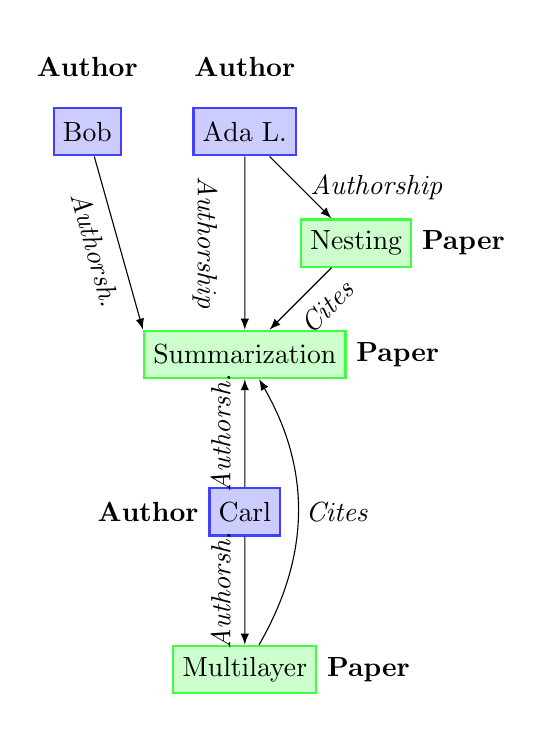
\begin{tikzpicture}[scale=1.1,every node/.style={minimum size=1cm,node distance=2cm},on grid]
	
	
	\tikzstyle{place}=[circle,thick,draw=blue!75,fill=blue!20,minimum size=6mm]
	\tikzstyle{red place}=[place,draw=red!75,fill=red!20]
	\tikzstyle{green place}=[place,draw=green!75,fill=green!20]
	\tikzstyle{transition}=[rectangle,thick,draw=black!75,
	fill=black!20,minimum size=4mm]
	
		\node  (w1) {};
		\node [place,rectangle] (ada1) [above of=w1,label=above:\textbf{Author}] {Ada L.};
		\node [place,rectangle] (bob) [left of=ada1,label=above:\textbf{Author}] {Bob};
		\node [green place,rectangle] (nest) [below right of=ada1,label=right:\textbf{Paper}] {Nesting};
		\node [green place,rectangle] (sum1) [below left of=nest,label=right:{\textbf{Paper}}] {Summarization};
		\node (g) [below of=sum1] {};
		\draw[-latex] (ada1) -- (nest) node [right,midway] {\textit{Authorship}};
		\draw[-latex] (ada1) -- (sum1) node [near end, midway,sloped,below] {\textit{Authorship}};
		\draw[latex-] (sum1) -- (nest) node [midway,below,sloped,yshift=.2cm] {\quad\textit{Cites}};
		\node [place,rectangle] (carl) [below of=sum1,label=left:\textbf{Author}] {Carl};
		\draw[-latex] (carl) -- (sum1) node [near end, midway,sloped,above,yshift=-.2cm] {\textit{Authorsh.}};
		\node [green place,rectangle] (multi) [below of=carl,label=right:{\textbf{Paper}}] {Multilayer};
		\draw[-latex] (carl) -- (multi) node [near end, midway,sloped,above,yshift=-.2cm] {\textit{Authorsh.}};
		\draw[-latex] (multi) edge [bend right] (sum1) node [right,sloped,yshift=2cm,xshift=.3cm] {\quad\textit{Cites}};
		\draw[-latex] (bob) -- (sum1.north west) node [near end, midway,sloped,below,yshift=.2cm] {\textit{Authorsh.}};	

	
	\end{tikzpicture}
\end{document}
